\documentclass[GBK,winfonts,a4paper,10pt]{ctexart}
\usepackage{fancyhdr}
\usepackage{indentfirst}
\usepackage{graphics}
\usepackage{enumerate}
\usepackage{framed}
\usepackage{amsmath}
\usepackage{graphicx}
\usepackage{setspace}
\usepackage{hyperref}
\usepackage{mdwlist}
\usepackage{algorithm}
\usepackage{algorithmic}
\usepackage{listings}
\usepackage{xcolor}
\usepackage{marvosym,listings,etoolbox}
\usepackage{geometry}

\lstset{numbers=left, numberstyle=\small, keywordstyle=\color{blue!70}, commentstyle=\color{red!50!green!50!blue!50}, frame=shadowbox, rulesepcolor=\color{red!20!green!20!blue!20},escapeinside=``, xleftmargin=2em,xrightmargin=2em, aboveskip=1em, literate={@}{\MVAt}1}

\patchcmd{\verb}{\dospecials}{\dospecials\atspecial}{}{}
\def\atspecial{\begingroup\lccode`~=`@
  \lowercase{\endgroup\let~}\MVAt
  \catcode`@=\active}
  


\newcommand{\tabincell}[2]{\begin{tabular}{@{}#1@{}}#2\end{tabular}}%
       
\lstdefinestyle{customc}{
  belowcaptionskip=1\baselineskip,
  breaklines=true,
  frame=single,
  xleftmargin=\parindent,
  language=C,
  showstringspaces=false,
  basicstyle=\fontsize{8pt}{8pt}\ttfamily,
  keywordstyle=\bfseries\color{green!40!black},
  commentstyle=\itshape\color{purple!40!black},
  identifierstyle=\color{blue},
  stringstyle=\color{orange},
  tabsize=4,
  numbers=none,
  mathescape=false,
}

\lstset{escapechar=@,style=customc}

\pagestyle{fancy}
\hypersetup{pdfborder=0 0 0}

\usepackage{clrscode}

\usepackage{latexsym}

\begin{document}

\rhead{}
\lhead{}
\cfoot{\thepage}
\renewcommand{\footrulewidth}{0.4pt}
%\renewcommand{\thesection}{}
\renewcommand{\algorithmicrequire}{\textbf{Input:}}
\renewcommand{\algorithmicensure}{\textbf{Output:}}
\setlength{\tabcolsep}{2pt}

\setlength{\parindent}{2em}

\thispagestyle{fancy}


\title{Operating System MIT 6.828 JOS Lab3 Report}
\author{Computer Science \\ ChenHao(1100012776) }
\date{\today}
\maketitle

\thispagestyle{fancy}

\tableofcontents

\newpage

\begin{section}{ Part A: User Environments and Exception Handling }
\par
lsof -i:xxxx    (xxxx是被占用的端口,得到占用端口的进程的PID)

\begin{subsection}{ Exercise 1 }
\par
分配物理内存和创建虚拟内存映射给envc,类似Lab2即可。
\begin{lstlisting}[language=C]
	envs = (struct Env *) boot_alloc(NENV * sizeof(struct Env));

// ... ...

    boot_map_region(kern_pgdir,
                    UENVS,
                    ROUNDUP(NENV * sizeof(struct Env), PGSIZE),
                    PADDR(envs),
                    PTE_U);
\end{lstlisting}
\end{subsection}

\begin{subsection}{ Exercise 2 }
\par
pmap只对内核进行了内存管理,而对于每个进程,都用有一个独立的内存空间,并且每个进程看起来都拥有整个内存空间,因此我们需要对进程也进行虚拟内存的管理,以及管理如何创建进程和进程的切换的问题。

\begin{subsubsection}{env\_init}
\par
env\_init类似page\_init,用来初始化NENV个进程管理结构,并且用单向链表来组织空闲的Env。其中要求env\_free\_list初始指向\&envs[0]。似乎这个的原因是在init.c中其会执行envs[0]。
\begin{lstlisting}[language=C]
void
env_init(void)
{
	// Set up envs array
	// LAB 3: Your code here.
    uint32_t i;
    env_free_list = envs;
    for (i = 0; i < NENV; i++) {
        envs[i].env_id = 0;
        envs[i].env_status = ENV_FREE;
        if (i + 1 != NENV)
            envs[i].env_link = envs + (i + 1);
        else 
            envs[i].env_link = NULL;
    }

	// Per-CPU part of the initialization
	env_init_percpu();
}
\end{lstlisting}
\end{subsubsection}

\begin{subsubsection}{env\_setup\_vm}
\par
env\_setup\_vm分配进程独立的Page Directory,即创建该进程的页目录。对于高于UTOP的虚拟地址PDE应与Kernel的页目录,对于低于UTOP的位置需要清0,这部分就是真正用户进程使用的页目录条目。
\par
为什么进程的页目录高于UTOP的虚拟地址的映射和Kernel的页目录一致?
\par
我觉得原因在于在内核管理进程的时候,在需用对进程使用的内存进行访问或者使用的时候就需要改用进程的Page Directory,但是同时还需要使用内核的代码或数据,因此保持一直可以保证这一点,不会造成错误和不必要的麻烦。而由于高于UTOP的虚拟地址的权限都是kernel权限的,因此在用户态的情况可以防止用户进行访问和修改,而且对于UTOP以上的内存对于用户进程是不允许访问的,这部分对于用户进程来说是不会使用的。
\begin{lstlisting}[language=C]
static int
env_setup_vm(struct Env *e)
{
	int i;
	struct PageInfo *p = NULL;

	// Allocate a page for the page directory
	if (!(p = page_alloc(ALLOC_ZERO)))
		return -E_NO_MEM;

    p->pp_ref++;
    e->env_pgdir = (pde_t *)page2kva(p);
    memcpy(e->env_pgdir, kern_pgdir, PGSIZE);
    memset(e->env_pgdir, 0, PDX(UTOP) * sizeof(pde_t));

	// UVPT maps the env's own page table read-only.
	// Permissions: kernel R, user R
	e->env_pgdir[PDX(UVPT)] = PADDR(e->env_pgdir) | PTE_P | PTE_U;

	return 0;
}
\end{lstlisting}
\end{subsubsection}

\begin{subsubsection}{region\_alloc}
\par
region\_alloc用于为进程分配物理内存,因此应该使用对应进程的页目录和页表。
\begin{lstlisting}[language=C]
static void
region_alloc(struct Env *e, void *va, size_t len)
{
    uint32_t addr = (uint32_t)ROUNDDOWN(va, PGSIZE);
    uint32_t end  = (uint32_t)ROUNDUP(va + len, PGSIZE);
    struct PageInfo *pg;
    // cprintf("region_alloc: %u %u\n", addr, end);
    int r;
    // cprintf("region_alloc: %u %u\n", addr, end);
    for ( ; addr != end; addr += PGSIZE) {
        pg = page_alloc(1);
        if (pg == NULL) {
            panic("region_alloc : can't alloc page\n");
        } else {
            r = page_insert(e->env_pgdir, pg, (void *)addr, PTE_U | PTE_W);
            if (r != 0) {
                panic("/kern/env.c/region_alloc : %e\n", r);
            }
        }
    }
    return;
}
\end{lstlisting}
\end{subsubsection}


\begin{subsubsection}{load\_icode}
\par
load\_icode将目标文件放入内存中,存放的虚拟内存的位置由目标文件指定。这个函数有两个需要注意的地方,第一个是首先使用region\_alloc分配对应虚拟地址的内存,而这个映射仅在该进程的页表中存在,在内核中是不存在的,因此在memcpy和memset的时候需要使用的该进程的页目录,而不应该使用内核的页目录。这个地方非常阴险,我一开始就掉进了这个陷阱中。
\par
第二个需要注意的地方就是需要将elf->e\_entry即目标文件的入口放入进程环境的eip中。
\begin{lstlisting}[language=C]
static void
load_icode(struct Env *e, uint8_t *binary, size_t size)
{
    struct Elf * elf = (struct Elf *)binary;
    if (elf->e_magic != ELF_MAGIC) {
        panic("error elf magic number\n");
    }
    struct Proghdr *ph, *eph;
    ph = (struct Proghdr *) ((uint8_t *) elf + elf->e_phoff);
    eph = ph + elf->e_phnum;

    lcr3(PADDR(e->env_pgdir));
    for (; ph < eph; ph++) {
        if (ph->p_type == ELF_PROG_LOAD) {
            region_alloc(e, (void *)ph->p_va, ph->p_memsz);
            memcpy((void *)ph->p_va, binary + ph->p_offset, ph->p_filesz);
            memset((void *)(ph->p_va) + ph->p_filesz, 0, ph->p_memsz - ph->p_filesz);
        }
    }
    e->env_tf.tf_eip = elf->e_entry;

    lcr3(PADDR(kern_pgdir));
    region_alloc(e, (void *)(USTACKTOP - PGSIZE), PGSIZE);

    return;
}
\end{lstlisting}
\end{subsubsection}


\begin{subsubsection}{env\_create}
\par
这个函数需要做就是将代码导入内存中,需要分两布:第一创建进程的地址空间的页目录以及设置环境变量,第二是将目标文件的代码导入内存中。
\begin{lstlisting}[language=C]
void
env_create(uint8_t *binary, size_t size, enum EnvType type)
{
    struct Env * e;
    int r = env_alloc(&e, 0);
    if (r < 0) {
        panic("env_create: %e\n", r);
    }
    load_icode(e, binary, size);
    e->env_type = type;
    return;
}
\end{lstlisting}
\end{subsubsection}

\begin{subsubsection}{env\_run}
\par
只需要进行切换一下即可。遗留问题如果curenv的状态为别的状态怎么办?之后回来再来看好了。
\begin{lstlisting}[language=C]
void
env_run(struct Env *e)
{
    if (curenv != NULL) {
        // context switch
        if (curenv->env_status == ENV_RUNNING) {
            curenv->env_status = ENV_RUNNABLE;
        }
        // how about other env_status ? e.g. like ENV_DYING ?
    }
    curenv = e;
    curenv->env_status = ENV_RUNNING;
    curenv->env_runs++;
    
    lcr3(PADDR(curenv->env_pgdir));

    env_pop_tf(&curenv->env_tf);    
	panic("env_run not yet implemented");
}
\end{lstlisting}
\end{subsubsection}

\par
gdb得到结果顺利到达int \$0x30处。
\end{subsection}

\begin{subsection}{ Exercise 3 }
\end{subsection}

\begin{subsection}{ Exercise 4 }
\par
由IA-32手册知是否需要Error Code的情况:
\begin{center}
    \begin{tabular}{ | l | l | l |}
    \hline
Interrupt   &   ID   &   Error Code  \\ \hline
divide error	&	0	&	N	\\ \hline 				
debug exception &  1  & N	\\ \hline 
non-maskable interrupt	&	2	&	N	\\ \hline 
breakpoint	&	3	&	N	\\ \hline 
overflow		&	4	&	N	\\ \hline 
bounds check		&	5	&	N	\\ \hline 
illegal opcode	&	6	&	N	\\ \hline 
device not available		&	7	&	N	\\ \hline 
double fault				&	8	&	N	\\ \hline 
invalid task switch segment	&	10	&	Y	\\ \hline 
segment not present	&	11	&	Y	\\ \hline 
stack exception	&	12	&	Y	\\ \hline 
general protection fault	&	13	&	Y	\\ \hline 
page fault	&	14	&	Y	\\ \hline 
floating point error	&	16	&	N	\\ \hline 
aligment check	&	17	&	Y		\\ \hline 
machine check		&	18	&	N	\\ \hline 
SIMD floating point error		&	19	&	N	\\ \hline
    \end{tabular}
\end{center}

\begin{subsubsection}{ trapentry.S }
\par
trapentry.S就是设置各种终端的入口,以及进入中断后队进程状态的保护。于是在trapentry.S的.text段中设置对应入口的汇编即可,对于状态的保护即在栈中建Trapframe,根据inc/trap.h中的Trapframe结构,存放相应的寄存器,并将GD\_KD导入\%ds和\%es中,保存\%esp执行trap()函数。
\begin{lstlisting}[language=C]
.text
 /*
 * Lab 3: Your code here for generating entry points for the different traps.
 */
 	TRAPHANDLER_NOEC(vec0, T_DIVIDE)
 	TRAPHANDLER_NOEC(vec1, T_DEBUG)
 	TRAPHANDLER_NOEC(vec2, T_NMI)
 	TRAPHANDLER_NOEC(vec3, T_BRKPT)
 	TRAPHANDLER_NOEC(vec4, T_OFLOW)

 	TRAPHANDLER_NOEC(vec6, T_BOUND)
	TRAPHANDLER_NOEC(vec7, T_DEVICE)
 	TRAPHANDLER_NOEC(vec8, T_DBLFLT)

 	TRAPHANDLER(vec10, T_TSS)
 	TRAPHANDLER(vec11, T_SEGNP)
 	TRAPHANDLER(vec12, T_STACK)
 	TRAPHANDLER(vec13, T_GPFLT)
 	TRAPHANDLER(vec14, T_PGFLT) 

 	TRAPHANDLER_NOEC(vec16, T_FPERR)
 	TRAPHANDLER(vec17, T_ALIGN)
 	TRAPHANDLER_NOEC(vec18, T_MCHK)
 	TRAPHANDLER_NOEC(vec19, T_SIMDERR)

/*
 * Lab 3: Your code here for _alltraps
 */
_alltraps:
	pushl %ds
	pushl %es
	pushal

	movl $GD_KD, %eax
	movw %ax, %ds
	movw %ax, %es

	pushl %esp
	call trap
\end{lstlisting}
\end{subsubsection}

\begin{subsubsection}{ trap\_init }
\par
trap\_init为初始化IDT表,并将表头导入IDTR中。IDT表中的项如下图所示:
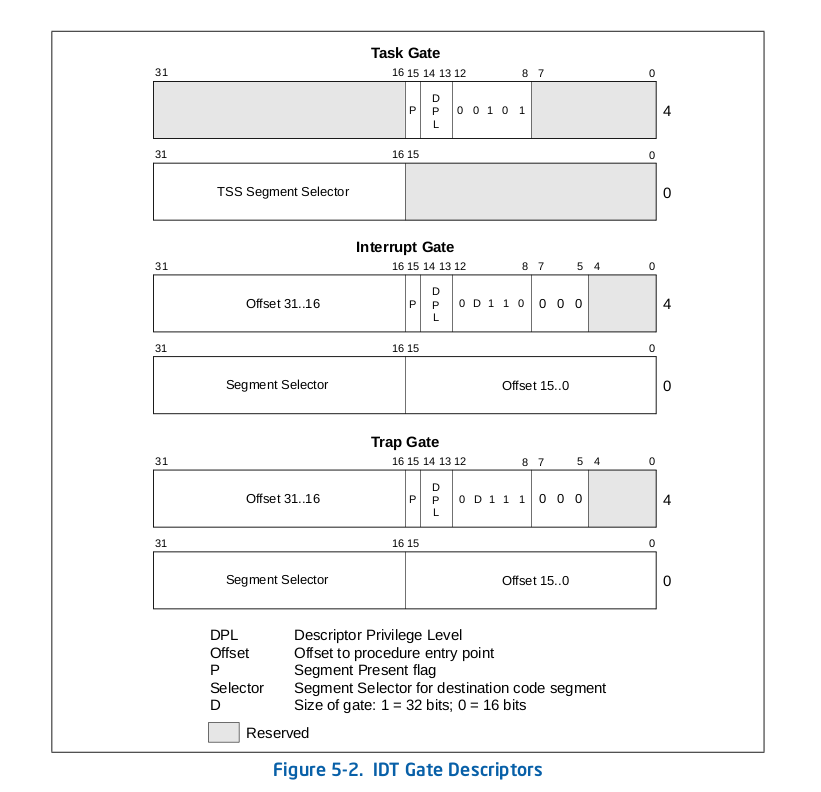
\includegraphics[scale=0.5]{IDTGateDescriptors.png}
因此将对应项传入SETGATE即可。
\begin{lstlisting}[language=C]
// In inc/mmu.h
// Set up a normal interrupt/trap gate descriptor.
// - istrap: 1 for a trap (= exception) gate, 0 for an interrupt gate.
    //   see section 9.6.1.3 of the i386 reference: "The difference between
    //   an interrupt gate and a trap gate is in the effect on IF (the
    //   interrupt-enable flag). An interrupt that vectors through an
    //   interrupt gate resets IF, thereby preventing other interrupts from
    //   interfering with the current interrupt handler. A subsequent IRET
    //   instruction restores IF to the value in the EFLAGS image on the
    //   stack. An interrupt through a trap gate does not change IF."
// - sel: Code segment selector for interrupt/trap handler
// - off: Offset in code segment for interrupt/trap handler
// - dpl: Descriptor Privilege Level -
//	  the privilege level required for software to invoke
//	  this interrupt/trap gate explicitly using an int instruction.
#define SETGATE(gate, istrap, sel, off, dpl) ...
// ----------------------------------------------------------------------------

void
trap_init(void)
{
	extern struct Segdesc gdt[];

	// LAB 3: Your code here.
	void vec0();
	void vec1();
	void vec2();
	void vec3();
	void vec4();
	void vec6();
	void vec7();
	void vec8();
	void vec10();
	void vec11();
	void vec12();
	void vec13();
	void vec14();
	void vec16();	
	void vec17();
	void vec18();
	void vec19();

	SETGATE(idt[0], 0, GD_KT, vec0, 0);
	SETGATE(idt[1], 0, GD_KT, vec1, 0);
	SETGATE(idt[2], 0, GD_KT, vec2, 0);
	SETGATE(idt[3], 0, GD_KT, vec3, 0);
	SETGATE(idt[4], 0, GD_KT, vec4, 0);

	SETGATE(idt[6], 0, GD_KT, vec6, 0);
	SETGATE(idt[7], 0, GD_KT, vec7, 0);
	SETGATE(idt[8], 0, GD_KT, vec8, 0);
	SETGATE(idt[10], 0, GD_KT, vec10, 0);
	SETGATE(idt[11], 0, GD_KT, vec11, 0);
	SETGATE(idt[12], 0, GD_KT, vec12, 0);
	SETGATE(idt[13], 0, GD_KT, vec13, 0);
	SETGATE(idt[14], 0, GD_KT, vec14, 0);

	SETGATE(idt[16], 0, GD_KT, vec16, 0);
	SETGATE(idt[17], 0, GD_KT, vec17, 0);
	SETGATE(idt[18], 0, GD_KT, vec18, 0);
	SETGATE(idt[19], 0, GD_KT, vec19, 0);

	// Per-CPU setup 
	trap_init_percpu();
}
\end{lstlisting}
执行,成功了!
\end{subsubsection}

\end{subsection}

\begin{subsection}{ Challenge 1 }
\par
好吧,看来Exercise4写挫了。。。得重写了
\par
实际上就是用data构造一个数组,每个数组都指向入口的地址,这样就可以完成了,我重新构建了三个宏,一个是对无error code的,一个是对有error code的,还有一个是对空着的无入口的中断。
\par
下面代码中'at'表示@,我的latex貌似显示不出来,查资料也解决不了。
\par
\begin{lstlisting}[language=C]
#define MYTH(name, num)			\
.text;		\
	.globl name;				\
	.type name, 'at'function;		\
	.align 2;			\
name:				\
	pushl $(num);		\
	jmp _alltraps;		\
.data;				\
	.long name


#define MYTH_NOEC(name, num)	\
.text;		\
	.globl name;				\
	.type name, 'at'function;		\
	.align 2;			\
name:				\
	pushl $0;			\
	pushl $(num);		\
	jmp _alltraps;		\
.data;	 			\
	.long name      

#define MYTH_NULL()		\
.data;				\
	.long 0
	

.data
.align 2
.globl vectors
vectors:
.text
	MYTH_NOEC(vec0, T_DIVIDE)
 	MYTH_NOEC(vec1, T_DEBUG)
 	MYTH_NOEC(vec2, T_NMI)
 	MYTH_NOEC(vec3, T_BRKPT)
 	MYTH_NOEC(vec4, T_OFLOW)
 	MYTH_NULL()
 	MYTH_NOEC(vec6, T_BOUND)
	MYTH_NOEC(vec7, T_DEVICE)
 	MYTH_NOEC(vec8, T_DBLFLT)
 	MYTH_NULL()
 	MYTH(vec10, T_TSS)
 	MYTH(vec11, T_SEGNP)
 	MYTH(vec12, T_STACK)
 	MYTH(vec13, T_GPFLT)
 	MYTH(vec14, T_PGFLT) 
 	MYTH_NULL()
 	MYTH_NOEC(vec16, T_FPERR)
 	MYTH(vec17, T_ALIGN)
 	MYTH_NOEC(vec18, T_MCHK)
 	MYTH_NOEC(vec19, T_SIMDERR)
  	
    TRAPHANDLER_NOEC(vec48, T_SYSCALL)
\end{lstlisting}
\par
对于初始化trap\_init,只需要按照数组的方式处理即可。方便了很多。代码如下:
\par
\begin{lstlisting}[language=C]
void
trap_init(void)
{
	extern struct Segdesc gdt[];
    
    extern uint32_t vectors[];
    extern void vec48();
    int i;
    for (i = 0; i != 20; i++) {
    	if (i == T_BRKPT) {
    		SETGATE(idt[i], 0, GD_KT, vectors[i], 3);
    	} else {
    		SETGATE(idt[i], 0, GD_KT, vectors[i], 0);
    	}
    }
    SETGATE(idt[48], 0, GD_KT, vec48, 3);

	// Per-CPU setup 
	trap_init_percpu();
}
\end{lstlisting}
\end{subsection}

\begin{subsection}{ Question }
\par
1. 有的中断需要error code,有的中断不需要。同时无法保存对应的中断号。因此需要分开处理。
\par
2. 因为IDT中设置page fault只能允许内核产生这种终端,如果在用户态产生page fault则会触发general protection fault。
\par
如果用户可以随意产生page fault,则可能有恶意的进程疯狂产生page fault将整个内存空间占满。因此page fault只能在内核中处理。
\end{subsection}
\end{section}

\begin{section}{ Part B: Page Faults, Breakpoints Exceptions, and System Calls }
\begin{subsection}{ Exercise 5 \& Exercise 6}
\par
根据trapno来分配即可
\begin{lstlisting}[language=C]
    int r;
    switch (tf->tf_trapno) {
        case T_PGFLT:
        		page_fault_handler(tf);
            break;
        case T_BRKPT:
            monitor(tf); 
            break;
        default:
	        // Unexpected trap: The user process or the kernel has a bug.
	        print_trapframe(tf);
	        if (tf->tf_cs == GD_KT)
		        panic("unhandled trap in kernel");
	        else {
		        env_destroy(curenv);
		        return;
	        }
    }
\end{lstlisting}
\end{subsection}

\begin{subsection}{ Challenge 2 }
\par
这个challenge就是需要在breakpoint的情况下增加continue和single-step的指令来进行调试。
\par
对于continue非常简单,增加一个mon的函数,其直接恢复curenv的enviroment即可。
\par
\begin{lstlisting}[language=C]
int 
mon_continue(int argc, char **argv, struct Trapframe *tf)
{
    if (tf == NULL) {
        cprintf("Error: you only can use continue in breakpoint.\n");
        return -1;
    }
    
    tf->tf_eflags &= (~FL_TF);
    env_run(curenv);    // usually it won't return;
    panic("mon_continue : env_run return");
    return 0;
}
\end{lstlisting}
\par
为了方便之后的测试我改变了一下usr/breakpoint.c的程序:
\par
\begin{lstlisting}[language=C]
#include <inc/lib.h>

void
umain(int argc, char **argv)
{
	asm volatile("int $3");

    // my code:
    cprintf("hello from A\n");
    cprintf("hello from B\n");
 	cprintf("hello from C\n");   
}
\end{lstlisting}
\par
然后进行运行,输入continue,发现输出了hello from A, B, C并正常结束,说明成功了! \par
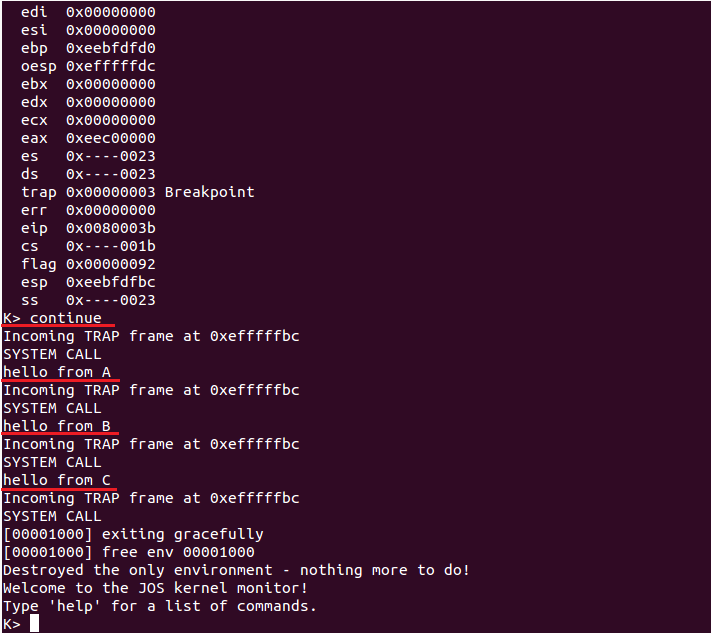
\includegraphics[scale=0.5]{continue.png}

\par
对于single-stepping则需要在tf\_eflags中设置TF位,然后恢复原进程的enviroment,当原进程执行完一条语句后会检查TF位,如果为1,则会自动触发一个int 1即debug exception。然后我们还需要在trap\_dispatch中处理T\_DEBUG, 为了偷懒,我直接使用了breakpoint的处理过程monitor(tf)。:) 
\par
\begin{lstlisting}[language=C]
\\ in trap_dispatch:
    switch (tf->tf_trapno) {
    		case T_DEBUG:
    			monitor(tf);
    			break;
    		...
    	}
    	
\\ in monitor.c
int 
mon_si(int argc, char **argv, struct Trapframe *tf)
{
    if (tf == NULL) {
        cprintf("Error: you only can use si in breakpoint.\n");
        return -1;
    }

    // next step also cause breakpoint interrupt
    tf->tf_eflags |= FL_TF;

    env_run(curenv);
    panic("mon_si : env_run return");
    return 0;
}
\end{lstlisting}
\par
我又改写了breakpoing.c的程序来测试
\par
\begin{lstlisting}[language=C]
void
umain(int argc, char **argv)
{
	asm volatile("int $3");

 	// my test for singal stepping
 	asm volatile("movl $0x1, %eax");
 	asm volatile("movl $0x2, %eax");
}
\end{lstlisting}
\par
我们来通过测试来观察\%eax的变化,为了方便看,我暂时注释掉print\_trapframe中的一些信息,只保留\%eax的值。结果如下:
\par
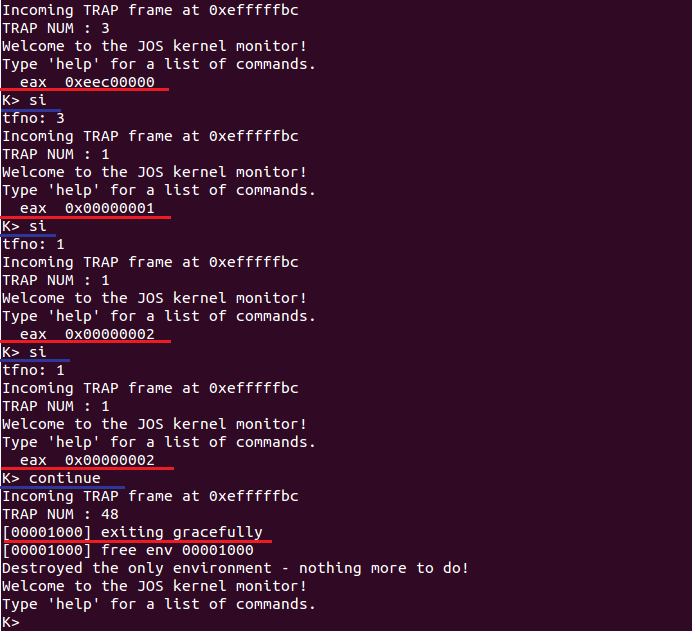
\includegraphics[scale=0.5]{step.png}
\par
完全符合预期,哈哈,搞定了!
\end{subsection}

\begin{subsection}{ Question }
\par
3. 由于breakpoint的陷阱是可以面向用户态的进程的,因此需要将IDT的特权位置设3,允许用户态进程使用。如果不设置则用户无法使用断点中断,当int 3的时候就会因为权限不足造成general protection fault。
\par
4. 这种机制有效限制了用户可以使用所有的中断而造成的问题,因此可以通过设置IDT的特权位来控制用户的中断操作。
\end{subsection}

\begin{subsection}{ Exercise 7 }
\par
系统调用的系统调用号会存在寄存器\%eax上,而接下来5个参数会存放在\%edx, \%ecx, \%ebx, \%edi, \%esi中,当系统调用结束后,其返回值会保存在寄存器\%eax上。
\par
lib/syscall.c中是用户调用系统调用的接口,里面也显示了不同系统调用的参数存放的位置,通过这个我们再根据系统调用号分开处理好系统调用即可。
\par
需要更改的地方有:
\par
(1)增加系统调用中断入口程序和将其地址加入IDT表中,注意特权位置要置为3,因为系统调用是提供给用户态进程使用的 
\par
(2)在中断的trap\_dispatch()中增加T\_SYSTEM的分配
(3)实现根据system call号来分发给不同的执行程序。
\begin{lstlisting}[language=C]
// trapentry.S:
    TRAPHANDLER_NOEC(vec48, T_SYSCALL)

// trap.c/trap_init
    void vec48();
    SETGATE(idt[48], 0, GD_KT, vec48, 3);    
    
// trap.c/trap_dispatch:
    switch (tf->tf_trapno) {
        case T_PGFLT:
        	if (tf->tf_cs == GD_KT)
        		panic("page fault in kernel");
        	else
        		page_fault_handler(tf);
            break;
        case T_BRKPT:
            monitor(tf); 
            break;
        case T_SYSCALL:
            r = syscall(tf->tf_regs.reg_eax, tf->tf_regs.reg_edx, tf->tf_regs.reg_ecx,
                        tf->tf_regs.reg_ebx, tf->tf_regs.reg_edi, tf->tf_regs.reg_esi);
            if (r < 0)
                panic("trap.c/syscall : %e\n", r);
            else
                tf->tf_regs.reg_eax = r;
            break;
        ...
    }
    
// syscall.c/syscall
// Dispatches to the correct kernel function, passing the arguments.
int32_t
syscall(uint32_t syscallno, uint32_t a1, uint32_t a2, uint32_t a3, uint32_t a4, uint32_t a5)
{
	// Call the function corresponding to the 'syscallno' parameter.
	// Return any appropriate return value.
	// LAB 3: Your code here.
    
    switch (syscallno) {
        case SYS_cputs:
            sys_cputs((char *)a1, (size_t)a2);
            return 0;
            break;
        case SYS_cgetc:
            return sys_cgetc();
            return 0;
            break;
        case SYS_getenvid:
            return sys_getenvid();
            break;
        case SYS_env_destroy:
            return sys_env_destroy(a1);
            break;
        dafult:
            return -E_INVAL;
	}
    panic("syscall not implemented");
}
\end{lstlisting}

\end{subsection}

\begin{subsection}{ Challenge 3 }

\end{subsection}

\begin{subsection}{ Exercise 8 }
\par
lib/entry.S是为创建的进程的入口,之后会跳转到libmain,之后会跳到相应的进程。在libmain需要记录该进程的环境。
\par
而我们有sys\_getenvid返回当前进程的envid号,ENVX(eid)可以得知其在envs的下标,这样就可以得到thisenv了。
\begin{lstlisting}[language=C]
	// set thisenv to point at our Env structure in envs[].
	// LAB 3: Your code here.
	thisenv = envs + ENVX(sys_getenvid());
\end{lstlisting}

\end{subsection}

\begin{subsection}{ Exercise 9 }
\par
如果在kernel下发生了page fault则说明这是一个bug,因此需要panic掉。思索一下加入kernel下发生page fault,而不panic会发生什么?
\par
因此需要在发生page fault的时候判断一下是用户态还是内核态下产生的page fault。
\par
\begin{lstlisting}[language=C]
// in trap.c/page_fault_handler

	// LAB 3: Your code here.
	if (tf->tf_cs == GD_KT)
    	panic("page_fault_handler : page fault in kernel\n");
\end{lstlisting}

\par
用户可能会通过中断访问不属于其空间的地址,例如printf一个内核的地址,或者创建超过字符串定义大小的内容等等。如果用户进程进行了这些操作,则直接杀掉它。
\par
填写检测所访问的虚拟地址是否在其内存空间内。
\begin{lstlisting}[language=C]
int
user_mem_check(struct Env *env, const void *va, size_t len, int perm)
{
	// LAB 3: Your code here.
	if (len == 0) return 0;		

	perm |= PTE_P;
	pte_t * pte;
	uint32_t va_now = (uint32_t)va;
	uint32_t va_last = ROUNDUP((uint32_t)va + len, PGSIZE);
	for (; ROUNDDOWN(va_now, PGSIZE) != va_last; va_now = ROUNDDOWN(va_now + PGSIZE, PGSIZE)) {
		if (va_now >= ULIM) {
			user_mem_check_addr = va_now;
			return -E_FAULT;
		}
		pte = pgdir_walk(env->env_pgdir, (void *)va_now, false);
		if (pte == NULL || ((*pte & perm ) != perm)) {
			user_mem_check_addr = va_now;
			return -E_FAULT;
		}
	}
	return 0;
}
\end{lstlisting}
\par
在sys\_cputs中加入:
\begin{lstlisting}[language=C]
	// LAB 3: Your code here.
    user_mem_assert(curenv, (void *)s, len, PTE_U);
\end{lstlisting}

\par
在kern/kdebug.c加入对usd, stabs, stabstr的检查。
\begin{lstlisting}[language=C]
		// Make sure this memory is valid.
		// Return -1 if it is not.  Hint: Call user_mem_check.
		// LAB 3: Your code here.
		if (user_mem_check(curenv, (void *)usd, sizeof(struct UserStabData), PTE_U) < 0) {
			return -1;
		}

		stabs = usd->stabs;
		stab_end = usd->stab_end;
		stabstr = usd->stabstr;
		stabstr_end = usd->stabstr_end;

		// Make sure the STABS and string table memory is valid.
		// LAB 3: Your code here.
		if (user_mem_check(curenv, (void *)stabs, (uint32_t)stab_end - (uint32_t)stabs, PTE_U) < 0) {
			return -1;
		}
		if (user_mem_check(curenv, (void *)stabstr, (uint32_t)stabstr_end - (uint32_t)stabstr, PTE_U) < 0) {
			return -1;
		}
\end{lstlisting}
\par
make run-breakpoint,backtrace,造成了page fault,具体如下图:
\par
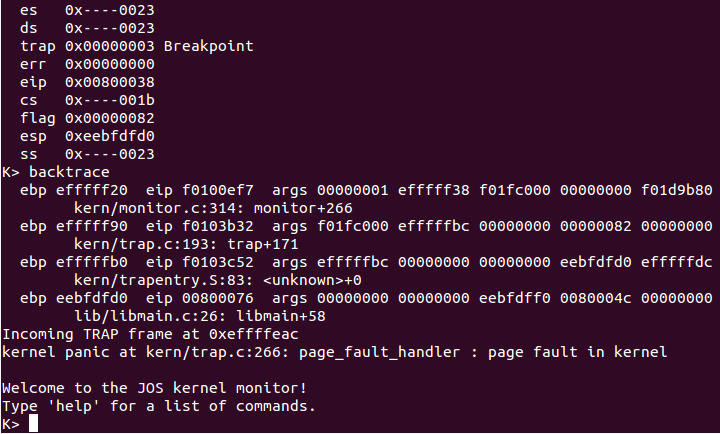
\includegraphics[scale=0.5]{backtrace.png}
\par
产生page fault的原因是其尝试访问了0xebfdfd0的位置读取上一个ebp,这个位置不在内核栈上,因此产生了page fault。
\par
为什么是0xebfdfd0呢?从env.c中的env\_alloc可知,初始设置栈为esp = USTACKTOP,这个位置是用户进程的栈空间的位置,这一段在内核中是没有映射的,所以当运行进程时,ebp保留的是用户进程的栈空间,因此当kernel尝试访问的时候就会造成page fault。	
\end{subsection}

\begin{subsection}{ Exercise 10 }
\par
似乎什么都没写就直接通过了。。通过看evilhello的其内核段写数据,我们确实在上面已经处理过了这种非法访问了。
\end{subsection}


\end{section}

\end{document}



















